\section{Motivation: Network of double integrators in presence of directed cycle}


\begin{frame}{Motivation}
	
	\begin{columns}[T,onlytextwidth]
		
		% Left column
		\begin{column}{0.48\textwidth}
			
			\begin{block}{Directed Acyclic Network}
				\begin{center}
					\begin{tikzpicture}[>=stealth, node distance=1.0cm]
						\foreach \i in {1,...,5}
						{
							\node[circle,draw=iitbblue,fill=iitbblue!10,
							minimum size=0.65cm] (n\i) at (\i*1.0,0) {\i};
						}
						\foreach \i [evaluate=\i as \j using int(\i+1)]
						in {1,...,4}
						{
							\draw[->,thick,iitbblue] (n\i) -- (n\j);
						}
					\end{tikzpicture}
				\end{center}
				\begin{itemize}
					\item Information flows along a directed chain.
					\item A directed spanning tree supports consensus.
				\end{itemize}
				\vspace{1em}
			\end{block}
			\begin{block}{Single-integrator agents}
				Directed cycles generally degrade the convergence rate, but do not necessarily destroy consensus.
			\end{block}
			
		\end{column}
		
		% Right column
		\begin{column}{0.48\textwidth}
			
			\begin{block}{Network with a Directed Cycle}
				\begin{center}
					\begin{tikzpicture}[>=stealth, node distance=1.0cm]
						\foreach \i in {1,...,5}
						{
							\node[circle,draw=iitbblue,fill=iitbblue!10,
							minimum size=0.65cm] (m\i) at (\i*1.0,0) {\i};
						}
						\foreach \i [evaluate=\i as \j using int(\i+1)]
						in {1,...,4}
						{
							\draw[->,thick,iitbblue] (m\i) -- (m\j);
						}
						\draw[->,very thick,mathred,bend left=25]
						(m5.south) to (m2.south);
					\end{tikzpicture}
				\end{center}
				\vspace{-0.5cm}
				\begin{itemize}
					\item Reverse edges introduce directed feedback loops.
					\item The Laplacian spectrum is modified.
				\end{itemize}
			\end{block}
			
			\begin{alertblock}{Double-integrator agents}
				Directed cycles can introduce instability when the
				velocity coupling gain is insufficient.
			\end{alertblock}
			
		\end{column}
		
	\end{columns}
	\vspace{0.15cm}
	\begin{center}
		\textbf{\color{iitbblue}
			How do directed cycles influence stability and performance,
			and how can consensus be guaranteed?}
	\end{center}
	
\end{frame}

\begin{frame}{The Double Integrator Consensus}
\vspace{-0.1cm}
	\textcolor{blue}{The system:}\vspace{-0.1cm} $$\dot{x}_i(t)=v_i(t),$$ $$\dot{v}_i(t)=u_i(t)$$
	\textcolor{blue}{Consensus} among double integrator, for any initial condition, is defined as:
	\vspace{-0.2cm}
	\begin{equation*}\label{SecondConsensus}
		\begin{array}{ll}
			\lim_{t \rightarrow \infty}||x_i(t)-x_j(t)||=0,\\
			\lim_{t \rightarrow \infty}||v_i(t)-v_j(t)||=0,\text{ } i,j \in \{1,2,\dots,N\}\\
		\end{array}
	\end{equation*}
	%where 
\vspace{-0.6cm}
\pause
	\begin{figure}
		\centering
		\begin{minipage}[]{0.2\linewidth}
			\centering
			\includegraphics[scale=0.5,keepaspectratio]{Images/Sapnning.eps}%\\ \textnormal{(a) Consensus achieved}
			\caption{Consensus achieved}
		\end{minipage}
		\hspace{1em}
		\begin{minipage}[]{0.2\linewidth}
			\centering
			\includegraphics[scale=0.5,keepaspectratio]{Images/Cycle.eps}%\\ \textnormal{(b) Consensus failed}
			\caption{Consensus failed}
		\end{minipage}
		\begin{minipage}[]{0.5\linewidth}
\vspace*{-0.3cm}
			%\centering
			\pause
			\textcolor{blue}{The proposed control law \footnotemark[1]}:
			\vspace*{-0.3cm}
			\small \begin{equation} \label{eq:agent-wise}
				u_i(t)=-\sum_{j=1}^{N}{w_{ij}[(x_j(t)-x_i(t))}+\gamma{(v_j(t)-v_i(t))}],
				\vspace{-0.3cm}
			\end{equation}
			\vspace{-0.3cm}
			\pause
			\begin{alertblock}{}
				This failure of consensus was owed to requirement of a higher value of the velocity coupling factor $\gamma$.	
			\end{alertblock}
		\end{minipage}
	\end{figure}
\vspace*{-0.5cm}
	where $x_i(t),v_i(t)\in \Rp$ denotes position and velocity of the $i^{th}$ agent in a $p$ dimensional space. $w_{ij}$ is the $(i,j)^{\rm th}$ entry of weighted adjacency matrix, and, $\gamma$ is called the \textbf{velocity coupling factor}.
\vspace{0.1cm}
{\footnotetext[1]{\textcolor{blue}{Ren W, Atkins E}, {\em Second-order consensus protocols in multiple vehicle systems with local interactions}, AIAA guidance, navigation, and control conference and exhibit 2005.}}	
\end{frame}

%\section{Consensus of Double Integrators in Presence of Directed Cycle}
\begin{frame}{Motivation: The Double Integrator Consensus}
Double integrator consensus is achieved if :
	\begin{itemize}
		\item Network has a \emph{directed spanning tree}.[Necessary but not sufficient] \\ \pause
		\item {$\gamma > \max_{i=2,\dots,n}\sqrt{\frac{2}{{\Re(\mu_i)}}}$ [Sufficient]~\footnotemark[1]}.\pause
		\item $\gamma > \max_{i=2,\dots,n}\frac{\Im(\mu_i)}{|\mu_i|\sqrt{{\Re(\mu_i)}}}$[Necessary \& Sufficient]~\footnotemark[2].
	\end{itemize}
	where $\mu_i$, are the non-zero eigenvalues of $\mathcal{L}$, and $\Re(.)$ and $\Im(.)$ represent real and imaginary parts.
	\pause
\vspace{-0.2cm}
	\begin{block}{Problem Statement}
		Consider a \textcolor{blue}{directed chain/path of double integrators containing one leader} node following the consensus protocol \eqref{eq:agent-wise}. Suppose a reverse edge is added to this network to result in a \textcolor{blue}{directed cycle} that may or may not include the leader (as shown below). Then, \textcolor{red}{can we design suitable \emph{local} strategy/strategies to ensure that consensus does not break down.}
	\end{block}
	\vspace{-0.1cm}
	\begin{figure}
		\centering
		\begin{minipage}[]{0.44\linewidth}
			\centering
			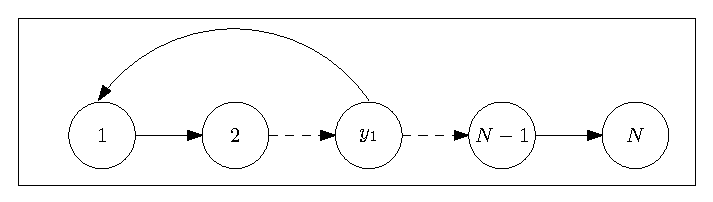
\includegraphics[scale=0.28, keepaspectratio]{Images/WithLeader.eps}\\
			\label{ChainLeader}
			\textnormal{\tiny(a) Directed Cycle With Leader}
		\end{minipage}
		\hspace{1em}
		\begin{minipage}[]{0.44\linewidth}
			\centering
			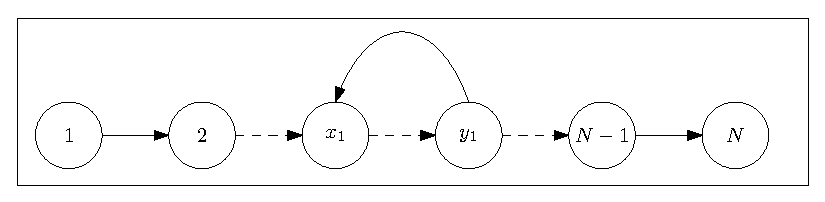
\includegraphics[scale=0.28, keepaspectratio]{Images/WithoutLeader.eps}\\
			\label{ChainWithoutLeader}
			\textnormal{\tiny(b) Directed Cycle Without Leader}
		\end{minipage}
	\end{figure}
	\vspace*{0.1cm}
	%\alt<1-2>{\let\thefootnote\relax\footnotetext{~}}
	{\footnotetext[1]{\textcolor{blue}{Ren W, Atkins E}, {\em Second-order consensus protocols in multiple vehicle systems with local interactions}, AIAA guidance, navigation, and control conference and exhibit 2005.}}
	%\alt<1-3>{\let\thefootnote\relax\footnotetext{~}}
	{\footnotetext[2]{\textcolor{blue}{Yu, Wenwu and Chen, Guanrong and Cao, Ming}, {\em Some necessary and sufficient conditions for second-order consensus in multi-agent dynamical systems}, Automatica 2010.}}		
	%\vspace{-0.5cm}	
\end{frame}


\begin{comment}
\begin{frame}{Problem 1}
	%\vspace{-0.2cm}
	\begin{block}{Problem Statement}
		Consider a \textcolor{blue}{directed chain/path of double integrators containing one leader} node following the consensus protocol \eqref{eq:agent-wise}. Suppose a reverse edge is added to this network to result in a \textcolor{blue}{directed cycle} that may or may not include the leader (as shown below).
	\end{block}
	\begin{figure}
		\centering
		\begin{minipage}[]{0.44\linewidth}
			\centering
			\includegraphics[height=1.2cm, keepaspectratio]{WithLeader.eps}\\
			\label{ChainLeader}
			\textnormal{(a) Directed Cycle With Leader}
		\end{minipage}
		\hspace{1em}
		\begin{minipage}[]{0.44\linewidth}
			\centering
			\includegraphics[height=1.2cm, keepaspectratio]{WithoutLeader.eps}\\
			\label{ChainWithoutLeader}
			\textnormal{(b) Directed Cycle Without Leader}
		\end{minipage}
	\end{figure} 
	\textcolor{blue}{The Objective: }Design suitable \emph{local} strategy/strategies to ensure that consensus does not break down, without adjusting any global variable such as $\gamma$.\\
	\begin{block}{Decentralized solution}
		By \emph{local} strategies, it is implied that the nodes forming the cycle should not be required to possess information about the complete Laplacian spectra.
	\end{block}
\end{frame}

\end{comment}


\begin{subframe}{Laplacian Structure}\label{LapStruct}
	%\vspace{-1cm}
	\textbf{Network Under consideration}:  -- A chain/directed path with $N$ nodes adhering to topological ordering,\\  --A single reverse edge from node $y_1$ to node $x_1$ ($y_1>x_1$) so that the length of the directed cycle is $\ell=y_1-x_1$.\\
	\textbf{Consequence}: Under topological ordering, the Laplacian will have a lower triangular structure:
	%\begin{figure}
		%\centering
		\begin{columns}
			\begin{column}{0.28\textwidth}
			~~	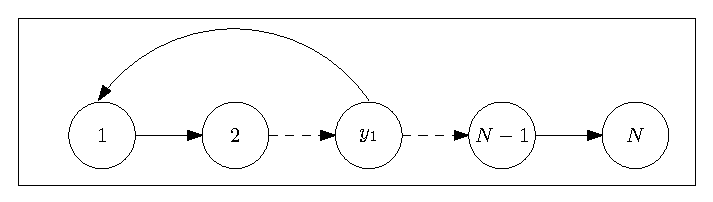
\includegraphics[scale=0.3, keepaspectratio]{Images/WithLeader.eps}
			\end{column}
			\hspace*{-0.5cm}
			\begin{column}{0.22\textwidth}
				$\mathcal{L}=\begin{bmatrix}
					\mathcal{C} & & 0 \\
					& & \\
					* & & \mathcal{L}_2
				\end{bmatrix}$,
			\end{column}
			
			%\centering
			%\label{ChainLeader}
			%\textnormal{(a) Directed Cycle With Leader}
		%\end{minipage}
	%	\hspace{0.5em}
		\begin{column}{0.28\textwidth}
			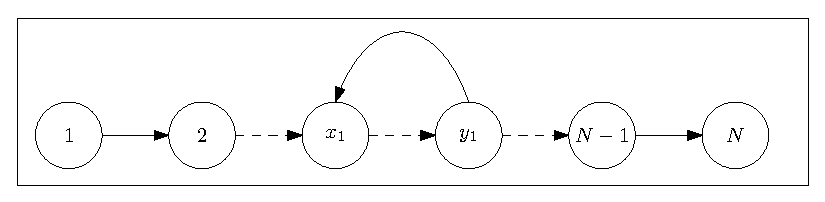
\includegraphics[scale=0.3, keepaspectratio]{Images/WithoutLeader.eps}
		\end{column}
		\begin{column}{0.22\textwidth}
			$\mathcal{L}=\begin{bmatrix}
				\mathcal{L}_1 & 0 & 0 \\
				* & \mathcal{C} & 0 \\
				* & * & \mathcal{L}_2
			\end{bmatrix}$
		\end{column}
		\end{columns}
			%\label{ChainWithoutLeader}
			%\textnormal{(b) Directed Cycle Without Leader}
%$		\end{minipage}
%	\end{figure}
	where $\mathcal{L}_2 \in \mathbb{R}^{(N-y_1) \times (N-y_1)}$,~~ $\mathcal{L}_1 \in \mathbb{R}^{(x_1-1) \times (x_1-1)}$ and $\mathcal{C} \in \mathbb{R}^{(\ell+1) \times (\ell+1)}$.\\
	\vspace{0.2cm}
	\textbf{Case 1:} \textcolor{blue}{With Leader}, $x_1=1 \implies \mathcal{L}_1$ vanishes and $\mathcal{C} \in \mathbb{R}^{y_1 \times y_1}$ exists.\\
	\textbf{Case 2:} \textcolor{blue}{On second reverse edge addition, Laplacian structure remains the same}.\\
	%\centering
	$$\mathcal{L}_2 \in \mathbb{R}^{(N-z_2) \times (N-z_2)},~~\mathcal{L}_1 \in \mathbb{R}^{(z_1-1) \times (z_1-1)},~~\mathcal{C} \in \mathbb{R}^{(z_2-z_1+1) \times (z_2-z_1+1)}$$\\ where $z_1=\min(x_1,x_2),z_2=\max(y_1,y_2)$.\\
	\textbf{Case 3:} Any change in the \textcolor{blue}{$\gamma$ bound is reflected by change in spectra of matrix $\mathcal{C}$}. 
	\hyperlink{BetterSuff}{\beamerbutton{Back}}
\end{subframe}
